\chapter{O Projeto} \label{int}
    O principal objetivo deste trabalho é estudar o desempenho duma rede LTE em vários cenários usando técnicas de
simulação de eventos discretos. Tal como no trabalho anterior, foi utilizado o simulador de rede ns-3 e realizamos três
estudos de forma a caracterizar melhor o funcionamento da rede LTE em diferentes cenários de utilização.

As simulações apresentadas foram largamente inspiradas nas realizadas no trabalho anterior sobre Wi-Fi e nos \textit{scripts}
de exemplo de LTE (lena-simple.cc e lena-simple-epc.cpp) que foram fornecidos juntamento com o simulador de rede ns-3.



\section{First Study - Throughput vs Distance} \label{ex1}
    Para este primeiro estudo , inspiramo-nos fortemente no homologo do trabalho anterior, e assim analisamos
a influência que a distância entre o equipamento do utilizador (ou "UE") e o nó de acesso possui no
\textit{throughput}.
Em teoria , seria de esperar que o aumento da distância entre um receptor e um transmissor resulte na queda gradual
do \textit{throughput} do equipamento do utilizador , juntamente com a diminuição do "Signal to Noise Ratio" (SNR) ou , neste caso,
do "Signal to Interference plus Noise Ratio" (SINR) que é o que nos é fornecido na execução do script.

Para obter os resultados apresentados, criámos um eNodeB na posição de origem (0,0,0) e um equipamento de utilizador (UE) com distância 
variável conforme a iteração ("distância",0,0). Esta simulação foi baseada no scrip "lena-simples.cc" com a adição do \textit{override} da distância. Os dados
sobre o número de bit/s presentes no meio foram obtidos do ficheiro "DlRlcStats.txt" e os dados sobre o SINR obtidos do ficheiro "DlRsrpSinrStats.txt".


\begin{figure}[H]
    \centering
    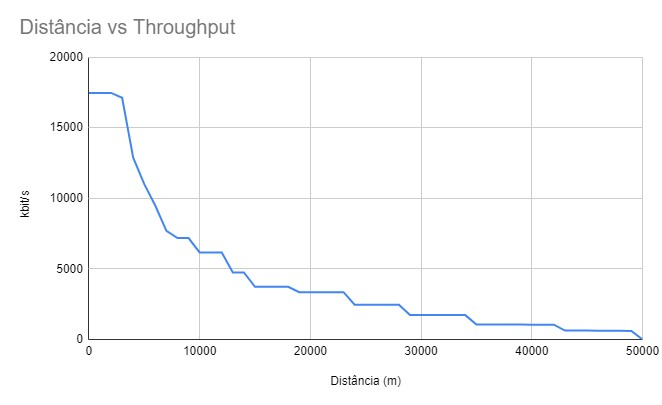
\includegraphics[width=.8\linewidth]{figs/fig1.jpg}
    \caption{\textit{throughput} vs Distância}
    \label{fig:1}
\end{figure}

Obtivemos um intervalo de confiança de +-1317m para um limite de confiança de 95\%.

\begin{figure}[H]
    \centering
    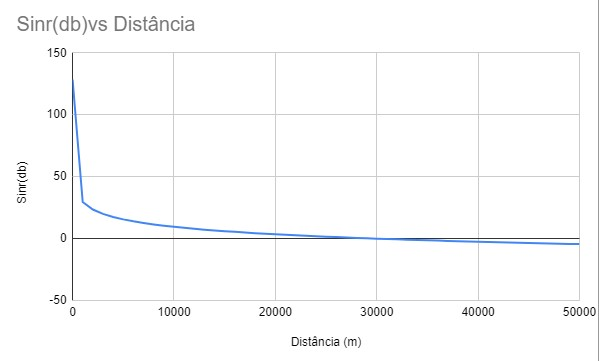
\includegraphics[width=.8\linewidth]{figs/fig2.jpg}
    \caption{Relação entre SINR(Sinal to Interference+Noise Ratio) e Distância}
    \label{fig:2}
\end{figure}
Obtivemos um intervalo de confiança de +-5,2 dB para um limite de confiança de 95\%.

Analisando os gráficos , podemos concluir que as nossas análises prévias se confirmam. O \textit{throughput} entra declinio apartir 
dos 3000m, ponto apartir do qual desce gradualmente. Entre os 49000m e os 50000m verifica-se uma acentuada descida para valores proximos de 0.

\clearpage


\section{Second Study-Throughput vs Number of UE's} \label{ex2}
    O segundo estudo deste trabalho é mais um vez baseado no seu equivalente do trabalho anterior.
Como tal , iremos avaliar os efeitos provocados no \textit{throughput} provocados pela 
presença de vários equipamentos de utilizador na rede. 
    É de esperar que com o aumento de utilizadores da rede , o \textit{throughput} vá diminuindo
gradualmente, uma vez que a capacidade da rede terá de ser distribuida de igual forma entre os vários
equipamentos.
    De forma a realizar esta experiência , colocámos um eNodeB na origem (0,0,0) e vários UE's distribuidos
numa circunferência com raio de 100m em torno do eNodeB, seguindo o mesmo procedimento que o segundo estudo 
da simulação de Wi-Fi.

\begin{figure}[H]
    \centering
    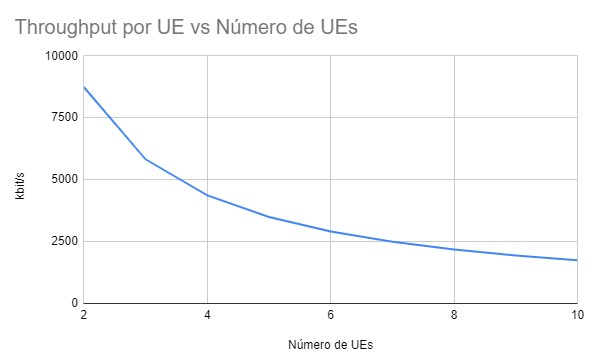
\includegraphics[width=.8\linewidth]{figs/fig3.jpg}
    \caption{\textit{throughput} vs Número de UE's}
    \label{fig:3}
\end{figure}
Obtivemos um intervalo de confiança de +-1490 kbit/s para um limite de confiança de 95\%.

    Facilmente confirmamos que os dados obtidos se alinham com o que era expectável. À medida
que aumentámos o número de equipamentos na rede , o \textit{throughput} de cada um deles vai diminuindo.
Para um maior numero de UE's , o acréscimo de cada equipamento representa uma diferença menor dado que a rede
já se encontra bastante dividida.


\clearpage





\section{Third Study - Throughput with Carrier Aggregation} \label{ex3}
    Para o terceiro estudo, queriamos observar a influência que a \textit{Carrier Aggregation (CA)} ou 
agregação de portadoras, tinha sobre o \textit{throughput} do sistema. Os testes foram realizados com a mesma
metodologia do primeiro estudo , em que íamos aumentando progressivamente a distância entre o
eNodeB e o equipamento do utilizador.
    A utilização de agregação de portadoras deverá permitir um aumento do \textit{throughput} de cada
utilizador , permitindo a utilização de vários blocos de frequência a um mesmo utilizador. Da mesma forma, 
quantos mais blocos estiverem a ser usados pelo utilizador , maior deverá ser o seu \textit{throughput}.



\begin{figure}[H]
    \centering
    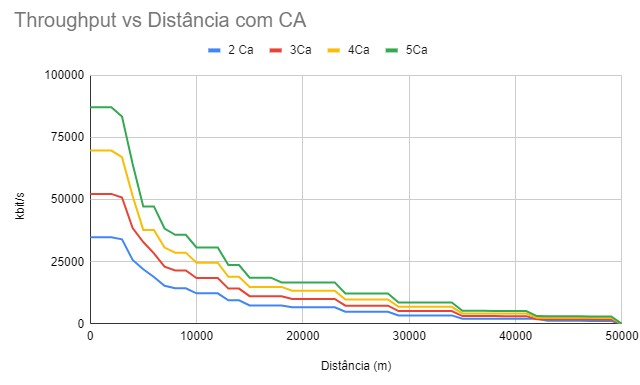
\includegraphics[width=.9\linewidth]{figs/fig8.jpg}
    \caption{Influência do uso de CA no \textit{throughput} vs Distância}
    \label{fig:4}
\end{figure}
\begin{table}[H]
    \begin{tabular}{lllll}
    CA & Intervalo de Confiança a 95\%    &  &  &  \\
    2  & +-2636m &  &  &  \\
    3  & +-3957m &  &  &  \\
    4  & +-5223m &  &  &  \\
    5  & +-6525m &  &  &  \\
    \end{tabular}
    \end{table}

    A figura 1.4 demonstra o que afirmamos anteriormente. Verificamos que o aumento do numero
de \textit{carriers} traduz-se num linear aumento do \textit{throughput} total, do que podemos 
concluir que a utilização de \textit{carrier aggregation} faz com que a informação seja dividida de igual 
forma pelos vários canais.

%\clearpage




